\documentclass{article}
\usepackage{graphicx}
\usepackage[margin=1.5cm]{geometry}
\usepackage{amsmath}

\begin{document}

\title{Monday Reading Assessment: Unit 6, Circular Motion}
\author{Prof. Jordan C. Hanson}

\maketitle

\section{Memory Bank}

\begin{itemize}
\item $\Delta s = r \Delta \theta$
\item $\omega = \frac{\Delta \theta}{\Delta t}$ ... Definition of angular velocity
\item $v = r\omega $ ... Relationship between tangential velocity and angular velocity a distance $r$ from the center
\end{itemize}

\section{Angular Displacement and Velocity}

\begin{enumerate}
\item 
\begin{figure}[ht]
\centering
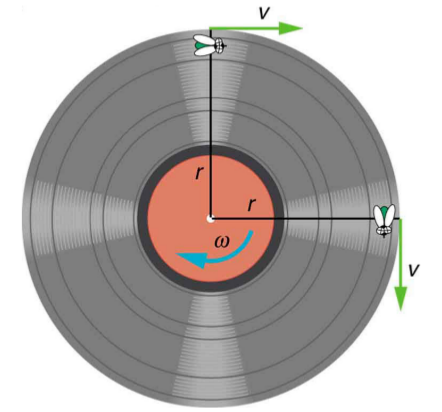
\includegraphics[width=0.25\textwidth]{record.png}
\caption{\label{fig:record} A record that is spinning counter-clockwise.}
\end{figure}

Suppose a record is spinning at 45 revolutions per minute, playing music (see Fig. \ref{fig:record}).  The radius is 15 cm.  Which of the following is true?
\begin{itemize}
\item A: A point near the edge (where the fly is) moves more slowly than one near the center. 
\item B: A point near the edge (where the fly is) moves faster than one near the center.
\item C: A point near the edge (where the fly is) moves at the same speed as one near the center.
\item D: A point near the edge has velocity, but the a point near the center does not have any velocity.
\end{itemize}
\item Suppose the radius is 15 cm, and the record spins at 45 revolutions per minute.  What is the velocity of the fly? \\ \vspace{2cm}
\item Suppose the radius is 15 cm, and we observe the velocity of the fly to be 0.35 m/s.  What is the angular velocity of the record?
\end{enumerate}

\end{document}
